\documentclass[xcolor={dvipsnames}]{beamer}
%\usepackage[utf8]{inputenc}
\usetheme{CambridgeUS}

%-------------------------------------------------------------------------------
%          -Packages nécessaires pour écrire en Français et en UTF8-
%-------------------------------------------------------------------------------
\usepackage[utf8]{inputenc}
\usepackage[frenchb]{babel}
\usepackage[T1]{fontenc}
\usepackage{lmodern}
\usepackage{textcomp}

%-------------------------------------------------------------------------------

%-------------------------------------------------------------------------------
%                          -Outils de mise en forme-
%-------------------------------------------------------------------------------
\usepackage{hyperref}
\hypersetup{pdfstartview=XYZ}
\usepackage{enumerate}
\usepackage{graphicx}
%\usepackage{multicol}
%\usepackage{tabularx}

%\usepackage{anysize} %%pour pouvoir mettre les marges qu'on veut
%\marginsize{2.5cm}{2.5cm}{2.5cm}{2.5cm}

\usepackage{indentfirst} %%pour que les premier paragraphes soient aussi indentés
\usepackage{verbatim}
%\usepackage[table]{xcolor}  
%\usepackage{multirow}
\usepackage{ulem}
%-------------------------------------------------------------------------------


%-------------------------------------------------------------------------------
%                  -Nécessaires pour écrire des mathématiques-
%-------------------------------------------------------------------------------
\usepackage{amsfonts}
\usepackage{amssymb}
\usepackage{amsmath}
\usepackage{amsthm}
\usepackage{tikz}
\usepackage{xlop}
\usepackage[output-decimal-marker={,}]{siunitx}
%-------------------------------------------------------------------------------


%-------------------------------------------------------------------------------
%                    - Mise en forme 
%-------------------------------------------------------------------------------

\newcommand{\bu}[1]{\underline{\textbf{#1}}}


\usepackage{ifthen}


\newcommand{\ifTrue}[2]{\ifthenelse{\equal{#1}{true}}{#2}{$\qquad \qquad$}}

\newcommand{\kword}[1]{\textcolor{red}{\underline{#1}}}


%-------------------------------------------------------------------------------



%-------------------------------------------------------------------------------
%                    - Racourcis d'écriture -
%-------------------------------------------------------------------------------

% Angles orientés (couples de vecteurs)
\newcommand{\aopp}[2]{(\vec{#1}, \vec{#2})} %Les deuc vecteurs sont positifs
\newcommand{\aopn}[2]{(\vec{#1}, -\vec{#2})} %Le second vecteur est négatif
\newcommand{\aonp}[2]{(-\vec{#1}, \vec{#2})} %Le premier vecteur est négatif
\newcommand{\aonn}[2]{(-\vec{#1}, -\vec{#2})} %Les deux vecteurs sont négatifs

%Ensembles mathématiques
\newcommand{\naturels}{\mathbb{N}} %Nombres naturels
\newcommand{\relatifs}{\mathbb{Z}} %Nombres relatifs
\newcommand{\rationnels}{\mathbb{Q}} %Nombres rationnels
\newcommand{\reels}{\mathbb{R}} %Nombres réels
\newcommand{\complexes}{\mathbb{C}} %Nombres complexes


%Intégration des parenthèses aux cosinus
\newcommand{\cosP}[1]{\cos\left(#1\right)}
\newcommand{\sinP}[1]{\sin\left(#1\right)}

%Fractions
\newcommand{\myfrac}[2]{{\LARGE $\frac{#1}{#2}$}}

%Vocabulaire courrant
\newcommand{\cad}{c'est-à-dire}

%Droites
\newcommand{\dte}[1]{droite $(#1)$}
\newcommand{\fig}[1]{figure $#1$}
\newcommand{\sym}{symétrique}
\newcommand{\syms}{symétriques}
\newcommand{\asym}{axe de symétrie}
\newcommand{\asyms}{axes de symétrie}
\newcommand{\seg}[1]{$[#1]$}
\newcommand{\monAngle}[1]{$\widehat{#1}$}
\newcommand{\bissec}{bissectrice}
\newcommand{\mediat}{médiatrice}
\newcommand{\ddte}[1]{$[#1)$}

%Figures
\newcommand{\para}{parallélogramme}
\newcommand{\paras}{parallélogrammes}
\newcommand{\myquad}{quadrilatère}
\newcommand{\myquads}{quadrilatères}
\newcommand{\co}{côtés opposés}
\newcommand{\diag}{diagonale}
\newcommand{\diags}{diagonales}
\newcommand{\supp}{supplémentaires}
\newcommand{\car}{carré}
\newcommand{\cars}{carrés}
\newcommand{\rect}{rectangle}
\newcommand{\rects}{rectangles}
\newcommand{\los}{losange}
\newcommand{\loss}{losanges}


%----------------------------------------------------

\title{Axes de symétrie d'une figure}
\author{}\institute{}


\AtBeginSection[]
{
	\begin{frame}
		\frametitle{Sommaire}
		\tableofcontents[currentsection, hideothersubsections]
	\end{frame} 
}

\begin{document}



\begin{frame}
  \titlepage
\end{frame}


\section{Rappels}

\begin{frame}
\frametitle{Symétrique d'un point M par rapport à une droite $(d)$}  
\framesubtitle{Définition}

\begin{block}<2->{Si M n'appartient pas à la droite $(d)$}
Dire que le point M' est le symétrique du point M par rapport à la droite $(d)$ signifie que la droite $(d)$ est la médiatrice du segment [MM'].
\end{block}

\begin{block}<3->{Si M appartient à la droite (d)}
Le symétrique M4 du point M par rapport à la droite (d) est lui-même.
C'est à dire, les points M et M' sont confondus.
\end{block}

\end{frame}

\section{Axes(s) de symétrie d'une figure}

\subsection{Définition}

\begin{frame}
\frametitle{Définition}  
\framesubtitle{}

Un \asym d'une figure $F$ est une \dte{d}  telle que le \sym\ de la \fig{F} par rapport à la \dte{d} est la \fig{F} elle-même.

\begin{columns}[c]

\begin{column}{2.2cm}
\begin{exampleblock}<2->{0 \asyms}
	\center{
\includegraphics[scale=0.25]{./img/stop}}
\end{exampleblock}	
\end{column}

\begin{column}{2.2cm}
	\begin{exampleblock}<3->{1 \asym }
		\center{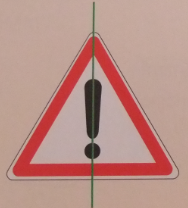
\includegraphics[scale=0.25]{./img/warn}}
	\end{exampleblock}	
\end{column}

\begin{column}{2.2cm}
	\begin{exampleblock}<4->{2 \asyms}
		\center{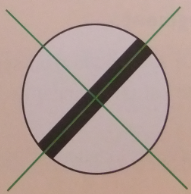
\includegraphics[scale=0.25]{./img/fin_limite}}
	\end{exampleblock}	
\end{column}

\begin{column}{2.2cm}
	\begin{exampleblock}<5->{4 \asyms}
		\center{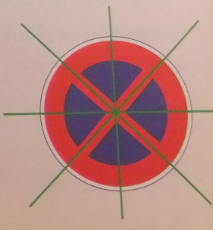
\includegraphics[scale=0.25]{./img/stationnement}}
	\end{exampleblock}	
\end{column}

\end{columns}


\end{frame}

\begin{frame}
\frametitle{Exemple}  
\framesubtitle{}
	\begin{exampleblock}{Une infinité d'\asyms}
		Un cercle admet une infité d'\asyms : \only<2>{toute droite passant par son centre.}
		
		\only<2>{\center{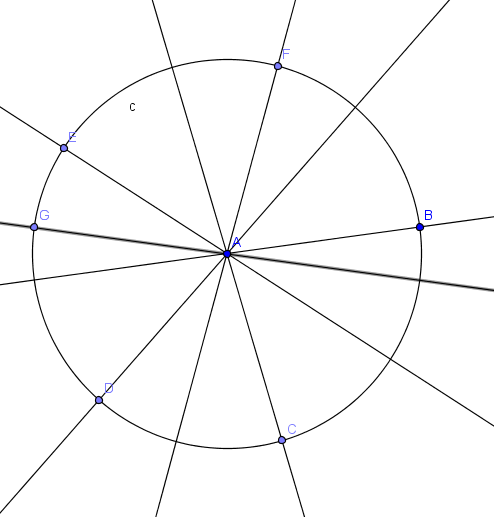
\includegraphics[scale=0.35]{./img/cercle}}}
	\end{exampleblock}
\end{frame}


\begin{frame}
\frametitle{Application}  
\framesubtitle{}

\begin{block}{Exercices}
	\begin{itemize}
		\item 35 p 212
		\item 36 p 212
		\item 37 p 212
	\end{itemize}
\end{block}
	
\end{frame}

\subsection{Axes de symétrie d'un segment}

\begin{frame}
\frametitle{Axe de symétrie d'un segment}  


\begin{alertblock}{Propriété}
	Un segment possède deux \asyms :
	\begin{itemize}
		\visible<2->{\item sa médiatrice}
		\visible<3->{\item la droite qui porte ce segment}
	\end{itemize}
\end{alertblock}

\center{\visible<2->{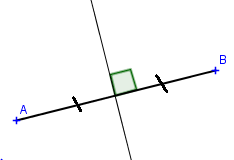
\includegraphics[scale=0.7]{./img/mediat}}}
\end{frame}

\begin{frame}
	\frametitle{Démonstration}  
	\framesubtitle{Médiatrice}

\begin{block}{On sait que}
\seg{AB} est un segment et $(d)$ est sa médiatrice.\pause
\end{block}

\begin{block}{Propriété}
	Si M n'appartient pas à la \dte{d}.
	Dire que le point M' est le symétrique du point M par rapport à la \dte{d} signifie que la \dte{d} est la médiatrice du segment \seg{MM'}.\pause
\end{block}

\begin{block}{Conclusion}
	B est le \sym\  de A par rapport à $(d)$ et A est le symétrique de B par rapport à $(d)$.
	Donc le symétrique du segment \seg{AB} par rapport à $(d)$ est lui-même.
	Donc la médiatrice (d) est un axe de symétrie du segment \seg{AB}.
\end{block}
\end{frame}

\begin{frame}
	\frametitle{Démonstration}  
	\framesubtitle{Droite portant le segment}
	
	\begin{block}{On sait que}
		\seg{AB} est un segment.\pause
	\end{block}
	
	\begin{block}{Propriété}
		Si M appartient à la \dte{d}.
		Le symétrique M' du point M par rapport à la \dte{d} est lui-même.
		C'est-à-dire, les points M et M' sont confondus.\pause
	\end{block}
	
	\begin{block}{Conclusion}
		A est le symétrique de A par rapport à la \dte{AB} et B est le symétrique de B par rapport à (AB).
		Donc le symétrique du segment [AB] par rapport à (AB) est lui-même.
		Donc la droite (AB) est un axe de symétrie du segment \seg{AB}.
	\end{block}
\end{frame}

\begin{frame}
	\frametitle{Application}  
	\framesubtitle{}
	
	\begin{block}{Exercices}
		\begin{itemize}
			\item 39 p 212
			\item 40 p 212
			\item 41 p 212
		\end{itemize}
	\end{block}
\end{frame}

\subsection{Axe de symétrie d'un angle}

\begin{frame}
\frametitle{Axe de symétrie d'un angle}  
\framesubtitle{}

\begin{alertblock}{Propriété (admise)}
	Un angle possède un \asym\ ;\pause  la droite qui porte sa bissectrice.
\end{alertblock}

\begin{columns}[c]
	
\begin{column}{7cm}
\begin{exampleblock}{Exemple}
	L'angle \monAngle{AOB} a pour \bissec\ la demi-droite \ddte{OC} et donc pour \asym\ la \dte{OC}.
\end{exampleblock}
\end{column}

\begin{column}{3cm}
	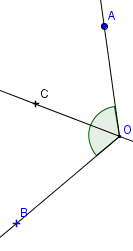
\includegraphics[scale=0.4]{./img/angle}
\end{column}

\end{columns}
\end{frame}

\begin{frame}
	\frametitle{Application}  
	\framesubtitle{}
	
	\begin{block}{Exercices}
		\begin{itemize}
			\item 43 p 212
			\item 44 p 212
			\item 45 p 212
		\end{itemize}
	\end{block}
\end{frame}

\section{Axes de symétrie de triangles}


\subsection{Le Triangle Isocèle}

\begin{frame}
\frametitle{Triangle Isocèle}  
\framesubtitle{}

\begin{columns}[c]
	

\begin{column}{7cm}

\begin{alertblock}{Propriété}
	Un triangle isocèle possède un axe de symétrie: \only<2->{la médiatrice de sa base.}
\end{alertblock}

\begin{block}<3>{Remarque}
	Cet axe de symétrie est aussi la bissectrice de l'angle au sommet principal.
\end{block}

\end{column}

\begin{column}{3cm}
	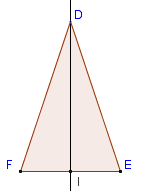
\includegraphics[scale=0.6]{./img/isocele}
\end{column}

\end{columns}

\end{frame}

\begin{frame}
\frametitle{Démonstration}  
\framesubtitle{}
	
\begin{columns}[c]
	
	
	\begin{column}{12cm}
		
		\begin{block}{On sait que}
			\small{Le triangle DEF est isocèle en D et que la \dte{DI} est la médiatrice du \seg{EF}.}\pause
		\end{block}
		
		\begin{block}{Propriété}
			\small{Si M appartient à la droite (d).
			Le symétrique M' du point M par rapport à la droite (d) est lui-même.
			C'est-à-dire, les points M et M' sont confondus.
			Si M n'appartient pas à la droite (d).
			Dire que le point M' est le symétrique du point M par rapport à la droite (d) signifie que la droite (d) est la médiatrice du segment [MM'].}\pause
		\end{block}
		
		\begin{block}{Conclusion}
			\small{Le symétrique du point D par rapport à la droite $(DI)$ est lui-même.
			Le symétrique de E est F et le symétrique de F est E.
			Donc le symétrique du triangle DEF est lui-même.
			Donc $(DI)$ est un axe de symétrie du triangle DEF.}
		\end{block}
		
	\end{column}
	
%	\begin{column}{2cm}
%		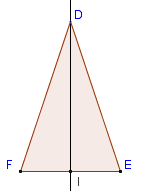
\includegraphics[scale=0.5]{./img/isocele}
%	\end{column}
	
\end{columns}
	
\end{frame}

\begin{frame}
	\frametitle{Application}  
	\framesubtitle{}
	
	\begin{block}{Exercices}
		\begin{itemize}
			\item 48 p 213
			\item 70 p 215
			\item 71 p 215
		\end{itemize}
	\end{block}
\end{frame}

\subsection{Le Triangle Équilatéral}

\begin{frame}
\frametitle{Le Triangle Équilatéral}  
\framesubtitle{}

\begin{columns}[c]
	
	
	\begin{column}{6cm}
		
		\begin{alertblock}{Propriété (admise)}
			Un triangle équilatéral possède trois axes de symétrie : \only<2->{les médiatrices de ses côtés.}
		\end{alertblock}
		
		\begin{block}<3>{Remarque}
			Ces axes de symétrie sont aussi les bissectrices des angles.
		\end{block}
		
	\end{column}
	
	\begin{column}{4cm}
		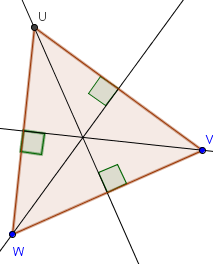
\includegraphics[scale=0.6]{./img/equilat}
	\end{column}
	
\end{columns}

\end{frame}

\begin{frame}
	\frametitle{Exemple}  
	\framesubtitle{}
	
	\begin{columns}[c]
		
		
		\begin{column}{7.5cm}
			
			\begin{block}{On sait que}
				Le triangle UVW est équilatéral. Les droites $(d1)$, $(d2)$ et $(d3)$ sont les médiatrices des côtés $[UV]$, $[VW]$ et $[UW]$.
			\end{block}
			
			\begin{block}<2->{Propriété}
				Un triangle équilatéral possède trois axes de symétrie: les médiatrices de ses côtés.
			\end{block}
			
			\begin{block}<3->{Conclusion}
				Donc ce sont les axes de symétries du triangle UVW.
			\end{block}
			
		\end{column}
		
		\begin{column}{3cm}
			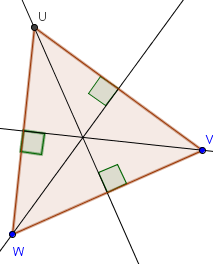
\includegraphics[scale=0.5]{./img/equilat}
		\end{column}
		
	\end{columns}
	
\end{frame}

\begin{frame}
	\frametitle{Application}  
	\framesubtitle{}
	
	\begin{block}{Exercice}
		\begin{itemize}
			\item 49 p 213
		\end{itemize}
	\end{block}
\end{frame}

\section{Axes de symétrie de quadrilatères usuels}

\subsection{Le Losange}

\begin{frame}
\frametitle{Le Losange}  
\framesubtitle{}

\begin{columns}[c]
	
	
	\begin{column}{9cm}
		
		\begin{block}{Définition}
			\small{Un losange est un quadrilatère qui a quatre côtés de même} longueur.
		\end{block}
		
		\begin{alertblock}<2->{Propriété (admise)}
			\small{Un losange possède deux axes de symétrie: ses diagonales.}
		\end{alertblock}
		
		\begin{alertblock}<3->{Propriété (admise)}
			\begin{small}
				
			 Si un quadrilatère est un losange, alors:
			 \begin{itemize}
			 	\item ses diagonales se coupent en leur milieu
			 	\item ses diagonales sont perpendiculaires
			 	\item ses angles opposés sont de même mesure
			 \end{itemize}
			 \end{small}
		\end{alertblock}
		

		
	\end{column}
	
	\begin{column}{2cm}
		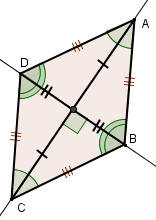
\includegraphics[scale=0.5]{./img/losange}
	\end{column}
	
\end{columns}

\end{frame}

\begin{frame}
	\frametitle{Application}  
	\framesubtitle{}
	
	\begin{block}{Exercices}
		\begin{itemize}
			\item 51 p 213
			\item 60 p 214
			\item 61 p 214
		\end{itemize}
	\end{block}
\end{frame}

\subsection{Le Rectangle}

\begin{frame}
\frametitle{Le Rectangle}  
\framesubtitle{}
blabla
\end{frame}

\subsection{Le Carré}

\begin{frame}
\frametitle{Le Carré}  
\framesubtitle{ST}
blabla
\end{frame}


\end{document}

\begin{frame}[label=lbl:]
\frametitle{}  
\framesubtitle{}
\end{frame}

\begin{block}{title}
contenu...
\end{block}

\begin{alertblock}{block title}
contenu...
\end{alertblock}


\begin{exampleblock}{block title}
contenu...
\end{exampleblock}


\begin{frame}
	\frametitle{Application}  
	\framesubtitle{}
	
	\begin{block}{Exercices}
		\begin{itemize}
			\item .. p ..
		\end{itemize}
	\end{block}
	
\end{frame}
